%%%%%%%%%%%%%%%%%%%%%%%%%%%%%%%%%%%%%%%%%%%%%%%%
%%%%%%%%%%%%%%%%%%%%%%%%%%%%%%%%%%%%%%%%%%%%%%%%%%
%%
%% Based one the "beamer-greek-two" template provided 
%% by the Laboratory of Computational Mathematics, 
%% Mathematical Software and Digital Typography, 
%% Department of Mathematics, University of the Aegean
%% (http://myria.math.aegean.gr/labs/dt/)
%%
%% Adapted by John Liaperdos, October-November 2014
%% (ioannis.liaperdos@gmail.com)
%%
%% Last update: 22/06/2017 (English Support)
%%
%%%%%%%%%%%%%%%%%%%%%%%%%%%%%%%%%%%%%%%%%%%%%%%%%%
%%%%%%%%%%%%%%%%%%%%%%%%%%%%%%%%%%%%%%%%%%%%%%%%%%
%%
\PassOptionsToPackage{unicode}{hyperref}
\PassOptionsToPackage{naturalnames}{hyperref}
\documentclass{beamer} 
%\usepackage{babel}
%\usepackage[utf8]{inputenc}


%%% FONT SELECTION %%%%%%%%%%%%%%%%%
%%% we choose a sans font %%%%%%%%%%
\usepackage{kmath,kerkis} 
%\usepackage[default]{gfsneohellenic} 
%%%%%%%%%%%%%%%%%%%%%%%%%%%%%%%%%%%%

\usepackage{color}
\usepackage{amsmath}
\usepackage{amssymb}
\usepackage[T1]{fontenc}
\usepackage[utf8]{inputenc}
\usepackage[brazil]{babel}
\usepackage{epstopdf}
\usepackage{graphicx}
\graphicspath{{./images/}}
\usepackage{tikz}
\usepackage{enumitem}
\usepackage{lmodern}
\usepackage{forloop}
\usepackage{calc}    % we need this to be able to multiply (*)
\usetikzlibrary{lindenmayersystems}
\usepackage{mathtools}
\usepackage{pgfplots}
\usepackage{hyperref}
\usetikzlibrary{math}
\pgfplotsset{compat=1.18} 


\hypersetup{
  colorlinks=true,
  linkcolor=blue,
  urlcolor=blue
}

%%
% load TEI-Pel - specific layout
\usepackage{TeiPel_En_Beamer_Layout}
\setTeipelLayout{draft,newlogo}% options: "draft", "newlogo"

\makeatletter
\def\moverlay{\mathpalette\mov@rlay}
\def\mov@rlay#1#2{\leavevmode\vtop{%
   \baselineskip\z@skip \lineskiplimit-\maxdimen
   \ialign{\hfil$\m@th#1##$\hfil\cr#2\crcr}}}
\newcommand{\charfusion}[3][\mathord]{
    #1{\ifx#1\mathop\vphantom{#2}\fi
        \mathpalette\mov@rlay{#2\cr#3}
      }
    \ifx#1\mathop\expandafter\displaylimits\fi}
\makeatother

\newcommand{\cupdot}{\charfusion[\mathbin]{\cup}{\cdot}}
\newcommand{\bigcupdot}{\charfusion[\mathop]{\bigcup}{\cdot}}

%%%%%%%%%%%%%%%%%%%%%%%%%%%%%%%%%%%%%%%%%%%%%%%%%%%%%%%%%%%%
% Thesis Info %%%%%%%%%%%%%%%%%%%%%%%%%%%%%%%%%%%%%%%%%%%%%%
%%%%%%%%%%%%%%%%%%%%%%%%%%%%%%%%%%%%%%%%%%%%%%%%%%%%%%%%%%%%
	% title
		\title{Testing}	
	% author 
    % (In the mandatory argument "{}", separate multiple
    % authors with "\and" - use "\\" for better author name formatting
    % in the title page. In the optional argument "[]" include all
	% author names, with no "\and" or text formatting macros.)
	% Example: 
    %\author[A. Author Albert Einstein]{Anthony Author \and Albert Einstein}
		\author[Kaique Oliveira]{by M. E. J. Newman}
	% supervisor	
                \supervisor{presented by Kaique M. M. Oliveira}
		%\supervisor{Orientador}{Prof. Dr.}{Luís Antônio C. dos Santos}
	% date
		\presentationDate{06 de Dezembro de 2023}
%%%%%%%%%%%%%%%%

\begin{document}

% typeset front slides
	\typesetFrontSlides

%%%%%%%%%%%%%%%%
% Your Slides Start here:
%%%%

%SECTION-----------------------------------------

\section{Introdução}


\begin{frame}{Introdução}

    \begin{exampleblock}{O que está por vir?}

        O objetivo é generalizar o modelo SIR de Kermack e McKendrick, um modelo 
        que assume população homogênea e taxa de contato e remoção fixas, para um modelo 
        onde em grafos com a distribuição de graus quaisquer, com taxas de infeção e remoção 
        sendo também distribuições quaisquer.
    
    \end{exampleblock}
    
\end{frame}


%%%%%%%%%%%%%%%%%%%%%%%%%%%%%%%%%%%%%%%%%%%%%%%%%%%%%%%%%%%%%%%%%%%%%%%%%%%%%%%%%%%%%%%%%%%%%%%%%%%%%%%

\section{O Modelo SIR}
\subsection{Descrição Matemática}
\begin{frame}{Modelo de Kermack e McKendrick}

    \begin{exampleblock}
        <1->{Modelo SIR}
        \begin{itemize}
            \item [$\bullet$] $s,i,r :=$ Percentual de Susceptíveis, Infectados e Removidos;
            \item [$\bullet$] $\beta, \gamma := $ Taxa média de Contato e de Remoção por tempo;
            \item [$\bullet$] O modelo é dado por
                $ 
                \begin{cases}
                    \frac{ds}{dt} &= -\beta i s; \\ 
                    \frac{di}{dt} &= \beta i s - \gamma i;  \\
                    \frac{dr}{dt} &= \gamma i \gamma. 
                \end{cases}
                $ 
                onde $s + i + r = 1$;
            \item [$\bullet$] Note que a taxa de infeção é homogênea, ou seja, a chance de um indivíduo
                infectado contaminar outra pessoa é sempre a mesma, independente da pessoa. 
            \item [$\bullet$] Soluções analíticas para o modelo são difíceis de encontrar, o que não 
                nos impede de tirar conclusões importantes sobre o comportamento do modelo.

        \end{itemize}

    \end{exampleblock} 
    
\end{frame}


%%%%%%%%%%%%%%%%%%%%%%%%%%%%%%%%%%%%%%%%%%%%%%%%%%%%%%%%%%%%%%%%%%%%%%%%%%%%%%%%%%%%%%%%%%%%%%%%%%%%%%%
\subsection{Número Básico de Reprodução}
\begin{frame}{Modelo de Kermack e McKendrick}


    \begin{exampleblock}
        <1->{Número Básico de Reprodução}

        \begin{itemize}
            \item [$\bullet$] Suponha que a população sucetível seja 1. O Número Básico de Reprodução 
                $R_0$ é o número médio de pessoas que a doença é transmitida antes da pessoa ser 
                imunizada. Note que, se $R_0>1$ a doença cresce, já se $R_0<0$, a doença descresce. 
                O limiar epidemiológico é definido quando $R_0 = 1$i.
            \item [$\bullet$] No modelo SIR, a doença cresce quando $\frac{di}{dt} > 0$. Supondo que 
                $s=1$ obtemos
                \[
                 0 < \frac{di}{dt} = \beta i s - \gamma i \iff 
                 0 < \beta i - \gamma i \iff 
                 i < \frac{\beta}{\gamma}i \iff 
                 0 < \frac{\beta}{\gamma}
                \]
                ou seja, $R_0 = \frac{\beta}{\gamma}$ denota o início da epidemia.
        \end{itemize}

    \end{exampleblock} 
    
\end{frame}

%%%%%%%%%%%%%%%%%%%%%%%%%%%%%%%%%%%%%%%%%%%%%%%%%%%%%%%%%%%%%%%%%%%%%%%%%%%%%%%%%%%%%%%%%%%%%%%%%%%%%%%
\subsection{Tamanho da Epidemia}
\begin{frame}{Modelo de Kermack e McKendrick}
    \begin{exampleblock}
	     <1->{Tamanho da Epidemia}
             \begin{itemize}
                 \item [$\bullet$] O tamanho da epidemia no modelo SIR nunca é igual a $1$ 
                     independente se $R_0 >> 1$ (onde $R_0 < \infty$), ou seja 
                    \[
                        s_\infty = 1 - r_\infty > 0, \qquad \forall R_0 \in \mathbb{R}.
                    \] 
                     A demonstração deste fato é envolvida, eis um modelo visual interativo para 
                     exploração: \href{https://www.geogebra.org/classic/pbddxfeh}{geogebra}
            
\begin{center}
    
\begin{tikzpicture}[scale=0.4]
  \begin{axis}[
    xlabel={Tempo},
    ylabel={População Normalizada},
    legend style={
      at={(0.5,-0.2)},
      anchor=north,
      legend columns=3,
      draw=none,
      /tikz/every even column/.append style={column sep=0.5cm}
    },
    cycle list name=color list,
    every axis plot/.append style={line width=1.5pt},
    ]
    
    \addplot table [y expr=\thisrow{S}/1000, mark=none, col sep=comma] {data.csv};
    \addlegendentry{Suscetíveis}
    \addplot table [y expr=\thisrow{I}/1000, mark=none, col sep=comma] {data.csv};
    \addlegendentry{Infeciosos}
    
    \addplot table [y expr=\thisrow{R}/1000, mark=none, col sep=comma] {data.csv};
    \addlegendentry{Removidos}
    
    \node[align=center, anchor=north east] at (axis description cs:1,0.8) {$\beta = 0.3$ \\ $\gamma = 0.1$};
    
  \end{axis}  
\end{tikzpicture}

\end{center}                
\end{itemize}
\end{exampleblock}

\end{frame}


%%%%%%%%%%%%%%%%%%%%%%%%%%%%%%%%%%%%%%%%%%%%%%%%%%%%%%%%%%%%%%%%%%%%%%%%%%%%%%%%%%%%%%%%%%%%%%%%%%%%%%%

\section{Modelo SIR em Grafos}
\subsection{Modelo de Configuração Percolado}

\begin{frame}{Modelo de Configuração Percolado}

\begin{exampleblock}
<1->{Modelo de Configuração}

\begin{itemize}
    \item[$\bullet$] Dada uma sequência de graus $(k_i)_{i \in \mathbb{N}}$, o grafo é selecionado de 
        forma uniforme e aleatória do conjunto de todos os grafos possíveis gerados por esta 
        sequência. A figura abaixo representa o algoritmo:

\begin{figure}
    \begin{center}

    % Draw nodes
    \begin{tikzpicture}[scale=1.2,transform shape]
        \node[circle,draw,minimum size=8mm] (A) at (0,0) {$i$};
        \node[circle,draw,minimum size=8mm] (B) at (2,0) {$j$};

        % Draw stubs for node A
        \draw (A.90) to[out=15,in=0] ++(0.5,0.5);
        \draw (A.45) to[out=45,in=180] ++(0.5,0.5);

        % Draw stubs for node B
        \draw (B.135) to[out=30,in=-45] ++(-0.5,0.5);
        \draw (B.90) to[out=30,in=-90] ++(0,0.5);
        \draw (B.45) to[out=0,in=-45] ++(0,0.5);

        \node at (-1.0,0) {\ldots};
        \node at (3.0,0) {\ldots};
    \end{tikzpicture}
    
    \end{center}
\end{figure}

\item[$\bullet$] No algoritmo acima, a chance de duas pontas se contectarem é sempre a mesma,
    independente das pontas. 
\item[$\bullet$] O próximo passo é generalizar a escolha da sequência $(k_i)_{i \in \mathbb{N}}$ 
    a partir de uma distribuição de graus $p_k$ de nossa escolha, qualquer que seja ela.

\end{itemize}

\end{exampleblock} 
    
\end{frame}


%%%%%%%%%%%%%%%%%%%%%%%%%%%%%%%%%%%%%%%%%%%%%%%%%%%%%%%%%%%%%%%%%%%%%%%%%%%%%%%%%%%%%%%%%%%%%%%%

\begin{frame}

\begin{exampleblock}
    <1->{Percolação por Ligações}

    \begin{itemize}
        \item[$\bullet$] Considere um grafo qualquer. Dada uma probabilidide $\phi$, o processo 
            de percolação por ligações é definido como o processo de ocupação de ligações 
            aleatoriamente com probabilidade $\phi$. Veja o exemplo abaixo.

            \begin{figure}
                \begin{center}
                    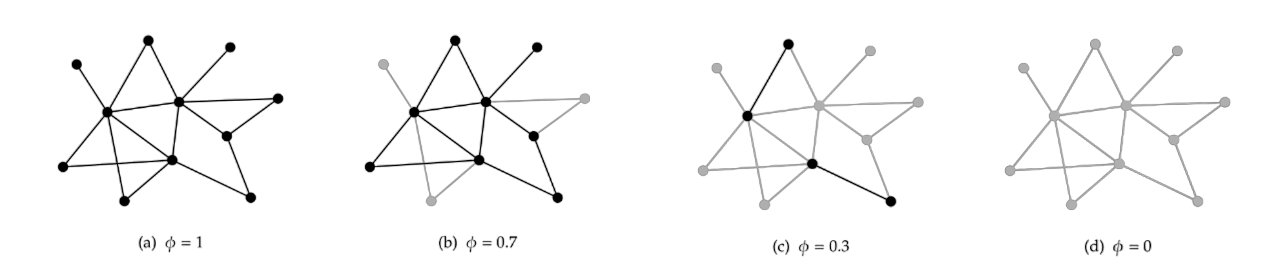
\includegraphics[scale=0.22]{images/grafo_branco.png}
                \end{center}
            \end{figure}
        \item[$\bullet$] Estamos interessados em analisar o espaço de todos os grafos de 
            configuração com distribuição de grau $p_k$ e percolação $T$, como definiremos
            a seguir

    \end{itemize}

\end{exampleblock}

\end{frame}

%%%%%%%%%%%%%%%%%%%%%%%%%%%%%%%%%%%%%%%%%%%%%%%%%%%%%%%%%%%%%%%%%%%%%%%%%%%%%%%%%%%%%%%%%%%%%

\begin{frame}

\begin{exampleblock}
    <1->{Taxa Média de Transmissão}

    \begin{itemize}
        \item[$\bullet$] Considere um par de indivíduos conectados $i$ e $j$, sendo $i$ infecioso
            e $j$ suscetível;
        \item[$\bullet$] Seja $r_{ij}$ a probabilidade de $i$ infectar $j$;
        \item[$\bullet$] Suponha que $i$ permanece infectado por um tempo total $\tau_i$;
        \item[$\bullet$] A probabilidade $1 - T_{ij}$ que $i$ não transmitirá a doença para $j$ é
            \[
                1 - T_{ij} = \lim_{\delta t \to 0} (1 - r_{ij} \delta t) \tau_i / \delta t = e^{- r_{ij} \tau_i }.
            \]
        \item[$\bullet$] Logo a probabilidade de Transmição é dada por
            \begin{align}
                T_{ij} = 1 -  e^{- r_{ij} \tau_i }. 
            \end{align}
    \end{itemize}       

\end{exampleblock}

\end{frame}

%%%%%%%%%%%%%%%%%%%%%%%%%%%%%%%%%%%%%%%%%%%%%%%%%%%%%%%%%%%%%%%%%%%%%%%%%%%%%%%%%%%%%%%%%%%%%


\begin{frame}

\begin{exampleblock}
    <1->{Taxa Média de Transmissão}

    \begin{itemize}
        \item[$\bullet$] Note que podemos escolher $r_{ij}$ e $\tau_i$ da maneira que quisermos. 
            Em particular, consideremos que $r_{ij}$ e $\tau_i$ são variáveis aleatórias 
            \textit{i.i.d} (independentes e identicamente distribuídas) escolhidas a partir das 
            distribuições $P(r)$ e $P(\tau)$, respectivamente. 
        
        \item[$\bullet$] Definimos $T$ como a média (valor esperado) de $T_{ij}$ sobre a distribuição de 
            probabilidade conjunto de $P(r)$ e $P(\tau)$, i.e 
        \begin{equation}
            T = \langle T_{ij} \rangle = 1 - \int_0 ^\infty \int_0 ^\infty P(r) P(\tau) e^{-r \tau} \, dr d\tau
        \end{equation}
        \item[$\bullet$] Uma conclusão que o valor $T$ nos fornece é que, globalmente 
            (uma parte não trivial da população), as diferenças locais (individuais) 
            são niveladas e não afetam o comportamento da doença em nível populacional.
    \end{itemize}


\end{exampleblock}

\end{frame}

%%%%%%%%%%%%%%%%%%%%%%%%%%%%%%%%%%%%%%%%%%%%%%%%%%%%%%%%%%%%%%%%%%%%%%%%%%%%%%%%%%%%%%%%%%%%%


%%%%%%%%%%%%%%%%%%%%%%%%%%%%%%%%%%%%%%%%%%%%%%%%%%%%%%%%%%%%%%%%%%%%%%%%%%%%%%%%%%%%%%%%%%%%%

\begin{frame}

\begin{exampleblock}
    <1->{Algumas Observações}

    \begin{itemize}
   
        \item[$\bullet$] Considere um surto de uma doença partindo de um indivíduo, em uma rede, 
            com transmissibilidade $T$. Marque como "ocupado" todas as ligações onde ocorre 
            transmissão. O tamanho total do surto é o tamanho do componente do grafo que o 
            individuo inicial participa. 

        \item[$\bullet$] O processo descrito acima é idêntico ao modelo de percolação por 
            ligações com taxa $T$ 

        \item[$\bullet$] Por fim, o nosso modelo epidemiológico será matematicamente descrito 
            pelo processo de percolação por ligações com taxa $T$ sobre uma rede condigurada. 


    \end{itemize}


\end{exampleblock}

\end{frame}

%%%%%%%%%%%%%%%%%%%%%%%%%%%%%%%%%%%%%%%%%%%%%%%%%%%%%%%%%%%%%%%%%%%%%%%%%%%%%%%%%%%%%%%%%%%%%

\subsection{Funções Geradas}
\begin{frame}{Funções Geradoras}

\begin{exampleblock}
    <1->{Distribuição do Grau}

    \begin{itemize}
   

        \item[$\bullet$] Considere a função geradora para a distribuição de graus $p_k$
            \[
                g_0(x)= \sum_{k=0}^\infty p_k x^k = p_0 + p_1 x + p_2 x^2 + ...
            \]
            Algumas propriedades da função geradora são
        \item[$\bullet$] $p_k = \frac{g^{(k)}(0)}{k!},$ \quad 
            $\bullet \langle 1 \rangle = g_0 (1) = 1,$ \quad 
           $ \bullet \langle k \rangle = g_0 ' (1), \quad $ ... 
        \item[$\bullet$] 
$\langle k^n \rangle = \left( z \frac{\delta}{\delta z} \right)^k g_0(z) \bigg|_{z=1}.$
        \item[$\bullet$] $g_{0 \left(\sum_{k=1}^n \mathrm{X}\right)} (z) = [ g_0 (z)] ^n$
    \end{itemize}


\end{exampleblock}

\end{frame}

%%%%%%%%%%%%%%%%%%%%%%%%%%%%%%%%%%%%%%%%%%%%%%%%%%%%%%%%%%%%%%%%%%%%%%%%%%%%%%%%%%%%%%%%%%%%%





\begin{frame}

\begin{exampleblock}
    <1->{Distribuição do Grau Excedente}

    \begin{itemize}

        \item[$\bullet$] Note que a distribuição de graus tendo seguido uma aresta é proporcinal 
            a $k p_k$. Logo, sua função geradora é dada por
            \[
                \frac{\sum k p_k x}{\sum k p_k} = x \frac{G_0 ' (x)}{ G_0 ' (1)}.
            \]
        \item[$\bullet$] Logo, a função geradora $G_1$ da distribuição de graus excedente é 
            \begin{equation}
                G_1(x) =  \frac{G_0 ' (x)}{ G_0 ' (1)} = \frac{G_0 ' (x)}{ z },
            \end{equation}
            onde $ z = G_0 ' (1)$.
    \end{itemize}


\end{exampleblock}

\end{frame}

%%%%%%%%%%%%%%%%%%%%%%%%%%%%%%%%%%%%%%%%%%%%%%%%%%%%%%%%%%%%%%%%%%%%%%%%%%%%%%%%%%%%%%%%%%%%%



\begin{frame}

\begin{exampleblock}
    <1->{Distribuição das Ligações Ocupadas}

    \begin{itemize}

        \item[$\bullet$] Faremos a mesma análise que a de cima mas, desta vez, sobre o modelo 
            de percolação de ligações. 
        
        \item[$\bullet$] A probabilidade de que um vértice tenha $m$ de suas $k$ arestas 
            ocupadas é dado por $\binom{k}{m} T^m (1-T)^{k-m}$. A distribuição 
            $G_0(x;T)$ do número de ligações ocupadas será dado por:
        \noindent
        \begin{align}
G_0(x;T) &= \sum_{m=0}^\infty \sum_{k = m}^\infty \binom{k}{m} T^m (1-T)^{k-m} x^m \\ 
         &= \sum_{k=0}^\infty p_k \sum_{m = 0}^k \binom{k}{m} T^m (1-T)^{k-m} x^m \\ 
         &= \sum_{k=0}^\infty p_k (1 - T + xT)^k
         = G_0 (1 +(x-1)T).
        \end{align}    


    \end{itemize}


\end{exampleblock}

\end{frame}

%%%%%%%%%%%%%%%%%%%%%%%%%%%%%%%%%%%%%%%%%%%%%%%%%%%%%%%%%%%%%%%%%%%%%%%%%%%%%%%%%%%%%%%%%%%%%



\subsection{Tamanho da epidemia}
\begin{frame}{Tamanho da epidemia}

\begin{exampleblock}
    <-1>{}
    \begin{itemize}

        \item[$\bullet$] Analogamente, a distribuição de ligações ocupadas excedentes é dada por 
            \begin{equation}
                G_1(x;T) = G_1(1 +(x-1)T).
            \end{equation}
    \end{itemize}

\end{exampleblock}

\begin{exampleblock}
    <-1>{Distribuição do Tamanho dos Surtos da Doença}
    \begin{itemize}

        \item[$\bullet$] Seja $P_s (T)$ a distribuição dos surtos 
            de tamanho $s$ para uma transmissibilidade $T$, o que equivalentemente é 
            a distribuição dos componentes no modelo de 
            percolação. Seja $H_0 (x; T)$ a sua função gerados correspondente, ou seja, 
            \begin{equation}
                H_0 (x; T)= \sum_{s=0}^\infty P_s (T) x^s.
            \end{equation}

    \end{itemize}
\end{exampleblock}


\end{frame}

%%%%%%%%%%%%%%%%%%%%%%%%%%%%%%%%%%%%%%%%%%%%%%%%%%%%%%%%%%%%%%%%%%%%%%%%%%%%%%%%%%%%%%%%%%%%%


\begin{frame}

\begin{exampleblock}
    <-1>{}
    \begin{itemize}
        \item[$\bullet$] Seguindo a mesma lógica que anteriormente, $H_1 (x;T)$ é a função geradora 
            para a distribuição dos componentes excedentes. É possível que $H_0$ e $H_1$ satisfazem: 
            \begin{align}
                H_1 (x; T) = x G_1 ( H_1 (x; T), T), \\
                H_0 (x; T) = x G_0 ( H_1 (x; T), T).
            \end{align}
        \item[$\bullet$] Solucionando as equações acima, analiticamente ou numericamente, é possível 
            encontrar a distribuição dos surtos $P_s (T)$ de tamanho dados por 
            \begin{equation}
                P_s (T) = \frac{H_0 ^{(k)}(0)}{k!}
            \end{equation}
    \end{itemize}

\end{exampleblock}



\end{frame}

%%%%%%%%%%%%%%%%%%%%%%%%%%%%%%%%%%%%%%%%%%%%%%%%%%%%%%%%%%%%%%%%%%%%%%%%%%%%%%%%%%%%%%%%%%%%%



\begin{frame}

\begin{exampleblock}
    <-1>{Média dos Surtos}
    \begin{itemize}
        \item[$\bullet$] Apesar de nem sempre conseguirmos encontrar a distrubuição $P_s (T)$ 
            dos surtos em forma fechada, a média $\langle s \rangle$ do tamanho dos surtos é 
            sempre possível de se encontrar, como segue:
            \begin{equation}
                \langle s \rangle = H_0 ' (1; T) = 1 + G_0 ' (1;T) H_1 ' (1;T). 
            \end{equation}
            Então 
            \begin{equation}
                \langle s \rangle = 1 + \frac{T G_0 ' (1) }{1 - T G_1 ' (1)} 
            \end{equation}
        \item[$\bullet$] Note que $\langle s \rangle$ diverge quando $T G_1 ' (1) = 1$, tal ponto 
            define o quando surto não ficará mais confinado a um número finito de casos (lembrando 
            que a nossa análise depende que $n>>1$).
    \end{itemize}
    
\end{exampleblock}



\end{frame}

%%%%%%%%%%%%%%%%%%%%%%%%%%%%%%%%%%%%%%%%%%%%%%%%%%%%%%%%%%%%%%%%%%%%%%%%%%%%%%%%%%%%%%%%%%%%%


\begin{frame}

\begin{exampleblock}
    <-1>{Tamanho da epidemia}
    \begin{itemize}
        \item[$\bullet$] As nossas definições de $H_0$ e $H_1$ das equações $(9)$ e $(10)$ 
            foram feitas supondo que não existem auto-ligações em um próprio nó ou múltiplas 
            ligações entre dois nós. Logo $H_0$ e $H_1$ estão definidos fora do componente gigante
            e podemos encontrar o tamanho $S(T)$ da epidemia fazendo
            \begin{equation}
                H_0 (1; T) = \sum_{s=0} ^\infty P_s = 1 - S(T).
            \end{equation}
            Então $S(T) = 1 - G_0 ( H_1 (1; T); T) $. Portanto, a probabilidade de um surto 
            com transmissão $T$ se tornar uma epidemia é simplesmente $S(T)$.
    \end{itemize}
    
\end{exampleblock}

\end{frame}

%%%%%%%%%%%%%%%%%%%%%%%%%%%%%%%%%%%%%%%%%%%%%%%%%%%%%%%%%%%%%%%%%%%%%%%%%%%%%%%%%%%%%%%%%%%%%




\begin{frame}
\begin{exampleblock} <-1>{Grau dos Infectados}
    \begin{itemize}
        \item[$\bullet$] Test


        \item[$\bullet$] Como $H_1$ só está definido fora do componente gigante, então $H_1 (1; T)$ é a 
            probabilidade de um nó não estar conectado a epidemia via um de seus vizinhos. É possível 
            mostrar que a média $z_{out}$ dos graus fora da epidemia é 
            \begin{equation}
                z_{out} = \frac{ H_1 (1; T)[1 - T + H_1 (1; T)]} {1 - S} z.
            \end{equation}
            E que a média $z_{in}$ dentro dos graus dentro da epidemia é 
            \begin{equation}
                z_{out} = \frac{ 1 - H_1 (1; T)[1 - T + H_1 (1; T)]} {S} z.
            \end{equation}
            Como esperado $z_{out} < z$ e $z_{in} \geq z$ e, também, se um nó tem grau $k$, 
            conforme $k \to \infty$ a change dele se infectar é 1.
    \end{itemize}
    
\end{exampleblock}

\end{frame}

%%%%%%%%%%%%%%%%%%%%%%%%%%%%%%%%%%%%%%%%%%%%%%%%%%%%%%%%%%%%%%%%%%%%%%%%%%%%%%%%%%%%%%%%%%%%%

\subsection{Exemplos}

\begin{frame}{Exemplo}
\begin{exampleblock}
    <-1>{Distribuição segundo Lei de Potência}
    \begin{itemize}

        \item[$\bullet$] Seja $p_k = C k^{\alpha} e ^{-k/ \kappa}, \quad k \geq 1$, 
            onde $C, \alpha, \kappa \in \mathbb{R}$ e $C = Li_\alpha (e^{-1/\kappa}.$

        \item[$\bullet$] Sejam $P(r)$ e $P(\tau)$ distribuições discretas e uniformes para $N$ nós e 
            valor fixo $ 0 \leq r \leq r_{max}$  e $0 \leq \tau \leq r_{max}$ escolhido.

        \item[$\bullet$] Então $T_{ij} = 1 -  (1 - r_{ij})^{\tau_i} = 1 - (1 - r)^\tau$, então.
        \item[$\bullet$] 
    $T = \langle T_{ij} \rangle = 1 - \sum_{r=0}^n \sum_{\tau=0}^n \left(  
    \frac{1}{r^{n-1}} \frac{1}{\tau^{n-1}}  (1 - r)^\tau \right)$

\item[$\bullet$] $G_0 (x) = \frac{\mathrm{Li} _\alpha ( x e ^{-1/\kappa})}{ \mathrm{Li}   _\alpha (  e ^{-1/\kappa})}$;
    \qquad $\bullet$ $G_0 (x) = \frac{\mathrm{Li} _{\alpha-1} ( x e ^{-1/\kappa})}{x L i _{\alpha-1} (  e ^{-1/\kappa})}$;
\item[$\bullet$]             
    $G_1 (x) = \frac{\mathrm{Li} _{\alpha-1} ( e ^{-1/\kappa})}{ \mathrm{Li}  _{\alpha-2} (  e ^{-1/\kappa})-  \mathrm{Li}  _{\alpha-1} (  e ^{-1/\kappa}) }$;
    \end{itemize}
    
\end{exampleblock}

\end{frame}

%%%%%%%%%%%%%%%%%%%%%%%%%%%%%%%%%%%%%%%%%%%%%%%%%%%%%%%%%%%%%%%%%%%%%%%%%%%%%%%%%%%%%%%%%%%%%


%%%%%%%%%%%%%%%%%%%%%%%%%%%%%%%%%%%%%%%%%%%%%%%%%%%%%%%%%%%%%%%%%%%%%%%%%%%%%%%%%%%%%%%%%%%%%

\begin{frame}{Exemplo}
\begin{exampleblock}
    <-1>{Distribuição segundo Lei de Potência}
    \begin{itemize}

        \item[$\bullet$] 
            $\langle s \rangle = 1  + \frac{ T [\mathrm{Li} _{\alpha-1} ( e ^{-1/\kappa})]^2}{ 
            \mathrm{Li}_\alpha (e^{-1/\kappa})[ (T+1) \mathrm{Li}  _{\alpha- 1} (  e ^{-1/\kappa})
            - T \mathrm{Li}  _{\alpha-2} (  e ^{-1/\kappa})]}; $

        \item[$\bullet$] 
            O tamanho $S$ da epidemia não pode ser achada de forma fechada, mas pode ser numericamente 
            aproximada, como visto anteriormente. A proxima figura representa a soluções aproximadas 
            para  $N = 100 000, \alpha = 2, \text{ para cada } \kappa = 5, 10 \text{ e } 15$. 
            Sob as mesmas condições, também é representada a simulação de $10 000$ surtos para cada 
            grafo gerado com para cada par $(P(r), P(\tau))$ onde $ P(r) = 0.1/N, 0.2/N, ..., 1/N$ e 
            $P(\tau) = 1/N, 2/N, ..., 10/N$. 

    \end{itemize}
    
\end{exampleblock}

\end{frame}

%%%%%%%%%%%%%%%%%%%%%%%%%%%%%%%%%%%%%%%%%%%%%%%%%%%%%%%%%%%%%%%%%%%%%%%%%%%%%%%%%%%%%%%%%%%%%



%%%%%%%%%%%%%%%%%%%%%%%%%%%%%%%%%%%%%%%%%%%%%%%%%%%%%%%%%%%%%%%%%%%%%%%%%%%%%%%%%%%%%%%%%%%%%

\begin{frame}{Exemplo}
\begin{exampleblock}
    <-1>{Distribuição segundo Lei de Potência}

    \begin{figure}
        \begin{center}
            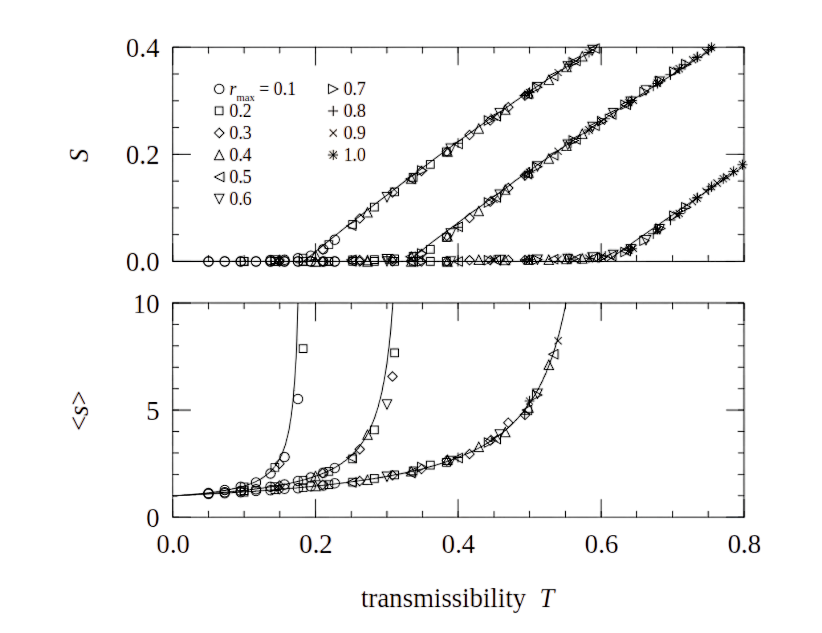
\includegraphics[scale=0.28]{images/epidemic_example.png}
        \end{center}
    \end{figure}
            

    
\end{exampleblock}

\end{frame}


\section{Referências}
\begin{frame}{Referências}


\begin{thebibliography}{3}

\beamertemplatearticlebibitems
\bibitem{PhysRevE.66.016128}
M. E. J. Newman,
\newblock Spread of epidemic disease on networks.
\newblock\emph{Phys. Rev. E},
\oldstylenums{66}(1):016128,
\oldstylenums{2002}.

\beamertemplatearticlebibitems
\bibitem{PhysRevE.64.026118}
M. E. J. Newman, S. H. Strogatz, and D. J. Watts,
\newblock Random graphs with arbitrary degree distributions and their applications.
\newblock\emph{Phys. Rev. E},
\oldstylenums{64}(2):026118,
\oldstylenums{2001}.


\beamertemplatebookbibitems
\bibitem{Author1990}M. E. J. Newman \newblock\emph{Networks}.\newblock
\textlatin{Oxford University Press, \oldstylenums{2018}}.

        \end{thebibliography}
\end{frame}

%%%%%%%%%%%%%%%%%%%%%%%%%%%%%%%%%%%%%%%%%%%%%%%%%%%%%%%%%%%%%%%%%%%%%%%%%%%%%%%%%%%%%%%%%%%%%



\end{document}

